%! TeX program = xelatex
%! TEX root = lecture1_slide.tex

\title{\texorpdfstring{$\lambda$}{λ}-Calculus}
\subtitle{Untyped \texorpdfstring{$\lambda$}{λ}-Calculus}
\begin{document}

\bgroup
  \usebackgroundtemplate{
\includegraphics[width=\paperwidth,height=\paperheight]{banner.pdf}}
  \begin{frame}[plain,noframenumbering]
    \maketitle
  \end{frame}
\egroup

%\begin{frame}[fragile]{Assessment guidelines}
%  \begin{description}
%    \item[Deadline] 17:00, 10 Aug
%    \item[Assessment] 
%      \begin{description}
%        \item[Assignment] (15\%)
%        \item[Exam] (100\%)
%      \end{description}
%    \item[Email] \texttt{liang.ting.chen.tw(at)gmail(dot)com}
%  \end{description}
%
%  \textbf{Please follow the instructions below.}
%
%  \begin{enumerate}
%    \item Use A4 paper.
%    \item Write down your name and student id. 
%    \item Be clear and brief.
%    \item Submit assignments in person or by email as \alert{PDF} with 
%      \begin{description}
%        \item[subject] \texttt{[FLOLAC] PL HW\%x\%}
%        \item[attachment] \texttt{PL-HW\%x\% - \%STDNO\% - \%NAME\%.pdf}
%        \item[body] (optional)
%      \end{description}
%  \end{enumerate}
%\end{frame}

\section{Untyped \texorpdfstring{$\lambda$}{λ}-Calculus: Introduction}
\begin{frame}[fragile]{The idea of anonymous functions}
Anonymous functions can be defined in many languages, e.g.,
\begin{description}
  \item[\Hask]
    \verb|\x f -> f x|
  \item[\OCaml]
    \verb|fun x f -> f x|
\end{description}

This type of expression is inspired by the \alert{$\lambda$-notation} introduced by Alan Turing's supervisor, Alonzo Church, who was seeking a foundational framework for mathematics.

\vfill

In $\lambda$-notation
\[
  \lam{x}e
\]
means `a function that maps the argument $x$ to expression $e$' where $x$ may appear in $e$.
E.g., the above examples can be expressed as
\[
  \lam{x\,f}f\;x
\]
\end{frame}

\begin{frame}{An example of $\lambda$-notation}
  The idea of function application in $\lambda$-notation is straightforward.

  For example, in high school we may say a function $f(x) \defeq x^2$ with the variable $x$ and write
  \[
    f(3) = 3^2 = 9
  \]

  In $\lambda$-notation, we write
  \[
    (\lambda x.\, x^2)\;3 = x^2 \subst{3}{x} = 3^2 = 9
  \]
  where $x^2\subst{3}{x}$ means `the \alert{substitution} of $3$ for $x$ in the expression $x^2$'. 
\end{frame}

\begin{frame}{What is $\lambda$-calculus}
  $\lambda$-calculus is a \emph{language of functions in $\lambda$-notation} consisting of three constructs:
\begin{description}
  \item[abstraction]
    functions can be introduced $\lam{x} t$

  \item[application]
    functions can be applied to an argument $t\;u$

  \item[variable]
    variables are terms
\end{description}
where a \emph{term} means a minimal unit of expression.

That is, every term in $\lambda$-calculus is in one and only one of the above forms.

$\lambda$-calculus can be understood as a programming language \emph{without} any built-in data types and suffices to define every computable function.
\end{frame}

\begin{frame}{Why should we study $\lambda$-calculus?}
  $\lambda$-calculus itself is a fruitful subject but it is also useful: 
  \begin{itemize}
    \item it serves as a prototype of programming languages which can be reasoned about \alert{mathematically} and \alert{rigorously};
    \item the methodology we develop to understand $\lambda$-calculus can be used to study and design other programming languages.
  \end{itemize}
  \vfill
  The common practice in PL research is to start with a variant of typed $\lambda$-calculus and a \emph{language feature} in question and investigate properties of this prototype language.

  \vfill 
  Moreover, $\lambda$-calculus has a strong connection with \emph{logic} and \emph{mathematics} which is a topic for another day.
\end{frame}

\begin{frame}{What to expect next?}
  For $\lambda$-calculus, we will consider following topics in programming language in a style of mathematical formalism.
  \begin{enumerate}
    \item How programs can be identified \emph{up to variable renaming}?
      E.g., $\lambda x.\, x$ should be `equal' to $\lambda y.\, y$.
    \item How do programs \emph{compute}?
      E.g., the application $(\lambda x.\, x)\;3$ of the identity to $3$ should compute to $3$.
    \item How programs can be identified \emph{computationally}?
      E.g.,
      \[
        (\lambda x.\, x)\;3 \quad\text{and}\quad (\lambda y.\, 3)\;10
      \]
      should be `computationally equal' as they should compute to the same term (but not each other).
    \item How to write programs in $\lambda$-calculus?
  \end{enumerate}
\end{frame}

\section{Untyped \texorpdfstring{$\lambda$}{λ}-Calculus: Statics}

\begin{frame}{Syntax of $\lambda$-calculus}
  To define the language of $\lambda$-calculus, we need a primitive notion of \emph{variables} first.
  Let us fix a \emph{countably infinite} set $V$ for variables.

  The set $\Lambda(V)$ of $\lambda$-terms over $V$ is defined \emph{inductively} as
  \begin{description}
    \item[variable] $x \in \Lambda(V)$ if $x$ is in $V$
    \item[application] $t@u \in \Lambda(V)$ if $t, u \in \Lambda(V)$
    \item[abstraction] $\lam{x}t$ if $x \in V$ and $t \in \Lambda(V)$
  \end{description}

  \vfill
  Each construct can be represented as a node in a tree where variables are leafs, e.g.,
  \begin{center}
    \begin{minipage}[t]{.32\textwidth}
      \centering
      \begin{tikzpicture}[
            level distance=0.75cm,
          level 1/.style={sibling distance=1cm},
        ]

        \node {$x$};
      \end{tikzpicture}
    \end{minipage}
    \begin{minipage}[t]{.32\textwidth}
      \centering
      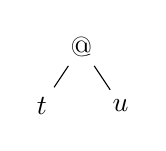
\begin{tikzpicture}[
            level distance=0.75cm,
          level 1/.style={sibling distance=1cm},
        ]

        \node {$@$}
          child { node {$t$} }
          child { node {$u$} };
      \end{tikzpicture}
    \end{minipage}
    \begin{minipage}[t]{.32\textwidth}
      \centering
      \begin{tikzpicture}[
            level distance=0.75cm,
          level 1/.style={sibling distance=2cm},
        ]

        \node {$\lambda x$}
          child { node {$t$} };
      \end{tikzpicture}
    \end{minipage}
  \end{center}
  for a variable $x$, an application $t@u$, and an abstraction $\lam{x}t$.
\end{frame}


\begin{frame}{Representing a term as an abstract syntax tree}
  The expression $\lam{x}(\lam{y}((x@y)@z))$ can be represented as
  \begin{center}
    \begin{tikzpicture}[
          level distance=1cm,
        level 1/.style={sibling distance=8cm},
        level 2/.style={sibling distance=5cm},
        level 3/.style={sibling distance=4cm}
      ]

      \node {$\lambda x$}
        child {node {$\lambda y$}
          child {node {$@$}
            child {node {$@$}
              child {node {$x$}}
              child {node {$y$}}
            }
            child {node {$z$}}
          }
        };
    \end{tikzpicture}
  \end{center}
  \begin{alertblock}{Important}
    Brackets `(' and `)' are not part of a term but are used for grouping a subterm.
  \end{alertblock}
\end{frame}

\begin{frame}{Formal justification}
  The validity of the expression can be justified by its very definition:
  \[
    \lam{x}(\lam{y}((x@y)@z))
  \]
  \begin{enumerate}
    \item $x$, $y$, and $z$ are in $V$, so $x$, $y$, $z$ are terms;
    \item $x$ and $y$ are terms, so $x@y$ is a term;
    \item $(x@y)@z$ is a term since $x@y$ is a term and $z$ is a term;
    \item {\small $\lam{y}((x@y)@z)$ is a term since $(x@y)@z$ is a term and $y$ is a variable;}
    \item {\footnotesize $\lam{y}((x@y)@z)$ is a term and $x$ is a variable, so $\lam{x}(\lam{y}((x@y)@z))$ is a term.}
  \end{enumerate}

  \begin{convention*}
    $@$ is omitted if a term is written as a sequence of symbols, so we write
    \[
      t\;u
      \qquad\text{instead of}\qquad
      t@u
    \]
  \end{convention*}
\end{frame}

\begin{frame}{The need for some conventions}
  For arithmetic expressions, we typically write
  \[
    3 * 4 + 7 *2 \qquad\text{to mean}\qquad (3 * 4) + (7 + 2)
  \]
  by the typical precedence convention.

  We'd also like to have some conventions to omit brackets without any ambiguity.
  E.g., one should be able to write
  \[
    \lam{x y}x\;y\;z \qquad\text{to mean}\qquad \lam{x}(\lam{y}((x\;y)\;z))
  \]
  since
  \begin{enumerate}
    \item multiple abstractions means a function with multiple arguments;
    \item applying a function to multiple arguments can be achieved via applying a function to a single argument and get another function which is applied to the next argument;
    \item applications occur more often than abstractions in a body.
  \end{enumerate}
\end{frame}
\begin{frame}{Conventions}
  \begin{description}
    \item[Consecutive abstractions]
      \[
        \lambda x_1\,x_2\,\ldots x_n.\, M \equiv \lambda x_1.\,(\lambda x_2.\,(\ldots (\lambda x_n.\, M)\ldots))
      \]
    \item[Consecutive applications]
      \[
        M_1\;M_2\; M_3\; \dots\;M_n \equiv (\dots((M_1\;M_2)\;M_3) \dots )\; M_n
      \]
    \item[Function body extends as far right as possible]
        $\lam{x}M\;N \quad\text{means}\quad \lambda x.\,(M\; N)$ instead of $(\lambda x.\,M)\; N$.
  \end{description}
  \begin{enumerate}
    \item $(x\;y)\;z \equiv x\;y\;z$
    \item $\lambda s.\,(\lambda z.\, (s \;z)) \equiv \lambda s\,z.\, s\;z$
    \item $\lambda a.\,(\lambda b.\, (a\;(\lambda c.\, a\; b))) \equiv \lambda a\,b.\, a\;(\lambda c.\, a\;b)$
    \item $(\lambda x.\, x)\;(\lambda y.\, y) \equiv (\lambda x.\, x)\;\lambda y.\, y$
  \end{enumerate}
\end{frame}
\begin{frame}{More Example}

  \begin{exercise*}
    Draw the corresponding abstract syntax tree for each of the following terms:
    \begin{enumerate}
      \item $x\;(y\;z)$
      \item $x\;y\;z$
      \item $\lam{sz}s\;z$
      \item $(\lambda x.\, x)\;(\lambda y.\, y)$
      \item $\lam{a b}a\;(\lam{c}a\;b)$
    \end{enumerate}
  \end{exercise*}
\end{frame}



\begin{frame}{Variable binding}
  Let's discuss an important notion of syntax: \emph{variable binding}.

  In the expression $f({\color{red}{x}}) = {\color{red}x}^2$, the variable $x$ in the expression $x^2$ is \alert{bound} to $x$ of $f$ and the \alert{meaning} of $f(x)$ is the same as $f({\color{red}y}) = {\color{red}y}^2$.

  Similarly, following expressions demonstrate the variable binding in various forms:
  \begin{enumerate}
    \item $\sum_{\alert{x} = 0}^{n} \alert{x}$
    \item $\int_{0}^{1} e^{\alert{y}}\; \mathrm{d}\alert{y}$
    \item $f({\color{red}x}, {\color{blue}y}) = {\color{red}x}^2 + {\color{blue}y}^2$
    \item \dots
    \item $\lambda {\color{red}y}.\,(\lambda {\color{blue}x}.\, {\color{red}y})$ means a function that takes an argument $y$ returns a constant function at $y$
    \item $\lambda {\color{red}x}.\,(\lambda {\color{blue}y}.\, {\color{blue}y})$ means a constant function that always returns an identity function
  \end{enumerate}
\end{frame}

\begin{frame}{Binding structure in an abstract syntax tree}
  The binding structure can be visualised in an abstract syntax tree:
  \begin{center}
    \begin{tikzpicture}[
          level distance=1.3cm,
        level 1/.style={sibling distance=8cm},
        level 2/.style={sibling distance=5cm},
        level 3/.style={sibling distance=4cm}
      ]

      \node (root) {$\lambda x$}
        child {node (lamy) {$\lambda y$}
          child {node {$@$}
            child {node {$@$}
              child {node (x) {$x$}}
              child {node (y) {$y$}}
            }
            child {node {$z$}}
          }
        };

        % Draw the arc from x to root
      \draw[red, ->, thick, dashed, bend left=60] (x) to (root);
      \draw[red, ->, thick, dashed, bend left=40] (y) to (lamy);

    \end{tikzpicture}
  \end{center}
\end{frame}

\begin{frame}{$\alpha$-equivalence: renaming of bound variables}
  It is common sense that renaming variables of a program should not alter its meaning: the point of having a name for a variable to look for where it applies to.

  \vfill
  Intuitively, two terms $t$ and $u$ are \alert{$\alpha$-equivalent}, written as
  \[
    t =_\alpha u
  \]
  if $t$ and $u$ have the same binding structure, \emph{regardless of their variable names}, in their abstract syntax trees.
  \vfill
  \begin{alertblock}{Quest}
    How to define $\alpha$-equivalence formally?
  \end{alertblock}
\end{frame}

\begin{frame}{First solution: de Bruijn representation}
  \begin{idea}
    The problem of variable renaming is the \emph{name}, so we may discard names and use indices $i'$ to represent variable bindings.
  \end{idea}

  The index $i'$ points to the $i$-th innermost $\lambda$-node from the variable: 
  \begin{center}
    \begin{minipage}{.4\textwidth}
      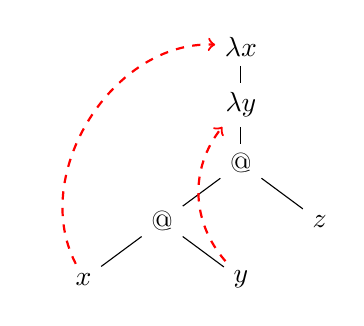
\begin{tikzpicture}[
            level distance=0.74cm,
          level 1/.style={sibling distance=6cm},
          level 2/.style={sibling distance=4cm},
          level 3/.style={sibling distance=2cm}
        ]
        \node (root) {$\lambda x$}
          child {node (lamy) {$\lambda y$}
            child {node {$@$}
              child {node {$@$}
                child {node (x) {$x$}}
                child {node (y) {$y$}}
              }
              child {node {$z$}}
            }
          };

        % Draw the arc from x to root
        \draw[red, ->, thick, dashed, bend left=60] (x) to (root);
        \draw[red, ->, thick, dashed, bend left=40] (y) to (lamy);
      \end{tikzpicture}
    \end{minipage}
    becomes
    \begin{minipage}{.4\textwidth}
      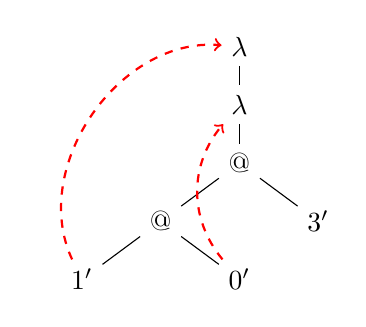
\begin{tikzpicture}[
            level distance=0.74cm,
          level 1/.style={sibling distance=6cm},
          level 2/.style={sibling distance=4cm},
          level 3/.style={sibling distance=2cm}
        ]
        \node (root) {$\lambda$}
          child {node (lamy) {$\lambda$}
            child {node {$@$}
              child {node {$@$}
                child {node (x) {$1'$}}
                child {node (y) {$0'$}}
              }
              child {node {$3'$}}
            }
          };

        % Draw the arc from x to root
        \draw[red, ->, thick, dashed, bend left=60] (x) to (root);
        \draw[red, ->, thick, dashed, bend left=40] (y) to (lamy);
      \end{tikzpicture}
    \end{minipage}
  \end{center}
  This representation is invented by a Dutch mathematician, N. G. de Bruijn, while implementing a language for formalising mathematics.
\end{frame}

\begin{frame}{Pros and cons of De Bruijn representation}
   
  \begin{description}
    \item[Good] This representation does solve many problems:
      \begin{enumerate}
        \item $\alpha$-equivalence coincides with syntactic equality, i.e.
          \[
            t =_\alpha u \iff t = u.
          \]
        \item Machine-readable.
        \item No variable renaming is involved.
      \end{enumerate}
    \item[Bad] `Don't throw the baby out with the bathwater'.
  \end{description}
\end{frame}

\begin{frame}{Second solution: Capture-avoidance renaming}
  \begin{idea}
    Using the nominal representation, we define $t =_\alpha u$ if variables $t$ and $u$ can be renamed `suitably' to exactly the same term.
  \end{idea}
  The problem with naive renaming is that a renamed variable might be \alert{captured} by another $\lambda$, breaking the binding structure.

  E.g., $y$ can be renamed to anything but $x$ in 
  \[
    \lambda x.\,(\lambda y.\, x \; y)
  \]
  to retain the same binding structure.

  Hence, variable renaming has to be constrained to variables that do not \alert{occur} in the term to avoid changing the binding structure.
  \begin{alertblock}{Quest}
    How to define the \alert{occurrence} of a variable and variable \alert{renaming}?
  \end{alertblock}
\end{frame}

\begin{frame}{Structural recursion over $\lambda$-terms}
  To define a function from $\lambda$-terms, we may use the '\alert{fold}':

  \begin{theorem*}
    Given a target set $X$ and functions
    \begin{align*}
      f_1 & \colon V \to X \\
      f_2 & \colon X \times X \to X \\
      f_3 & \colon V \times X \to X
    \end{align*}
    there exists a unique $\hat{f}\colon \Lambda(V)  \to X$ such that
    \begin{align*}
      \hat{f}\,x    & = f_1\,x \\
      \hat{f}(t\;u) & = f_2(\hat{f}\,t, \hat{f}\,u) \\
      \hat{f}(\lambda x.\, t) & = f_3(x, \hat{f}\,t)
    \end{align*}
  \end{theorem*}
\end{frame}

%\begin{frame}{Exercise: Height}
%
%The \emph{height} of a term is given informally as follows:
%\begin{enumerate}
%  \item the height of a variable is 1;
%  \item the height of an application is the maximum of the heights of its subterms plus 1;
%  \item the height of an abstraction is the height of its body plus 1.
%\end{enumerate}
%
%\begin{exercise*}
%  Define the height function $h\colon \Lambda(V) \to \mathbb{N}$ by structural recursion.
%\end{exercise*}
%\end{frame}

\begin{frame}{Variable occurrences}
  We define the set $\Var(t)$ of variables in a term $t$ by structural recursion with the target set $\mathcal{P}V$ and
\begin{align*}
  \Var_1(x) & = \{x\} \\
  \Var_2(S_1, S_2) & = S_1 \cup S_2 \\
  \Var_3(x, S) & =  \{x\} \cup S
\end{align*}
  That is, $\Var$ is a function from $\Lambda(V)$ to $\mathcal{P}V$ such that 
  \begin{align*}
    \Var(x) & = \{x\} \\
    \Var(t\;u) & = \Var(t) \cup \Var(u) \\
    \Var(\lam{x} t) & = \{x\} \cup \Var(t) 
  \end{align*}
  \vfill
  We say $x$ occurs in $t$ if $x \in \Var(t)$, i.e.\ $x$ appear in $t$ somewhere.
\end{frame}


\begin{frame}{Variable permutation}
  A \emph{transposition} $(x\, y)$ is a function that swaps $x$ and $y$ but fixes everything else, i.e.\
  \[
    (x\, y)\;z = 
    \begin{cases}
      y & \text{$z$ = $x$} \\
      x & \text{$z$ = $y$} \\
      z & \text{otherwise}
    \end{cases}
  \]
   \vfill
   The \emph{variable permutation} by a transportation $\pi = (y\,z)$ is defined by
   \begin{align*}
     \pi\cdot x     & = \pi\;x \\
     \pi\cdot(t\;u) & = (\pi\cdot t)\; (\pi\cdot u) \\
     \pi\cdot(\lambda x.\, t) & = \lambda (\pi\;x).\, (\pi\cdot t)
   \end{align*}
   \vfill
   E.g.,
  \[
    (z\,y) \cdot \lambda x.\,(\lambda y.\, y \; y) = \lambda x.\,(\lambda z.\, z \; z)
  \]
\end{frame}

\begin{frame}{Renaming of bound variables}
  Now we are ready to formulate what we mean by $\alpha$-equivalence

  \begin{definition}[$\alpha$-equivalence]
    $\alpha$-equivalence is a relation $t =_\alpha u$ between terms $t$ and $u$ defined inductively as
  \begin{multicols}{2}
    \begin{prooftree}
      \AXC{\vphantom{$M_1$}}
      \RightLabel{if $x \in V$}
      \UIC{$x =_\alpha x$}
    \end{prooftree}
    \begin{prooftree}
      \AXC{$t_1 \mathrel{=_\alpha} t_2$}
      \AXC{$u_1 \mathrel{=_\alpha} u_2$}
      \BIC{$t_1\;u_1 \mathrel{=_\alpha} t_2\;u_2$}
    \end{prooftree}
  \end{multicols}
  \begin{prooftree}
    \AXC{$(z\;x)\cdot t \mathrel{=_\alpha} (z\;y)\cdot u$}
    \RightLabel{if $z \not\in \Var(t, u)$}
    \UIC{$\lam{x}t \mathrel{=_\alpha} \lam{y}u $}
  \end{prooftree}
  \end{definition}
  The third case is the interesting one: $\lam{x}t$ and $\lam{y}u$ are equal up to renaming bound variables if the variables $x$ and $y$ can be swapped with a variable $z$ that does not exist in $t$ and $u$.
\end{frame}

\begin{frame}{An example of $\alpha$-equivalent terms}

  \begin{example}
    Show that $(\lambda y.\, y)\;z =_\alpha (\lambda x.\,x)\;z$.
  \end{example}

  \begin{proof}
    By definition
    \begin{prooftree}
      \AXC{}
      \UIC{$(y\;y)\cdot y \mathrel{=_\alpha} (y\; x)\cdot x$}
      \UIC{$\lambda y.\, y \mathrel{=_\alpha} \lambda x.\, x$}
      \AXC{}
      \UIC{$z \mathrel{=_\alpha} z$}
      \BIC{$(\lambda y.\, y)\;z \mathrel{=_\alpha} (\lambda x.\, x)\;z$}
    \end{prooftree}
  where $(y\;y)\cdot y = () \cdot y = y$ and $(y\;x)\cdot x = y$, so it follows that $(\lambda y.\, y)\;z \mathrel{=_\alpha} (\lambda x.\, x)\;z$.
  \end{proof}
\end{frame}


\begin{frame}{$\alpha$-equivalence is an equivalence}
  $\alpha$-equivalence satisfies the following properties
  \begin{description}
    \item[reflexivity] $t =_\alpha t$ for any term $t$;
    \item[symmetry] $u =_\alpha t$ if $t =_\alpha u$;
    \item[transitivity] $t =_\alpha v$ if $t =_\alpha u$ and $u =_\alpha v$. 
  \end{description}
  Easy to prove reflexivity and symmetry (try it!) but tricky to prove transitivity.
  \vfill
  We are mainly in interested in \alert{terms up to $\alpha$-equivalence}, as the name of a bound variable does not matter. 
  Hence, we consider $\lambda$-terms \emph{modulo} $\alpha$-equivalence, i.e.\
  \[
    [t]_{\alpha} = \{\, u \in \Lambda(V) \mid t =_\alpha u \,\}
  \]
  as well as the (quotient) set:
  \[
    \Lambda(V)/{=_\alpha} \defeq \{\, [t]_{\alpha} \mid t \in \Lambda(V) \,\}.
  \]
\end{frame}

\begin{frame}{Exercise}
Which of the following pairs are $\alpha$-equivalent? If so, prove it.
\begin{enumerate}
  \item $x$ and $y$ if $x \neq y$ 
  \item $\lambda x\,y.\, y$ and $\lambda z\,y.\, y$
  \item $\lambda x\,y.\, x$ and $\lambda y\,x.\, y$
  \item $\lambda x\,y.\, x$ and $\lambda x\,y.\, y$
\end{enumerate}
\vfill
\begin{block}{Challenge}
Is it true that $\alpha$-equivalent terms have the same de Bruijn representation?

Can you come up with a strategy to prove your conjecture?
\end{block}

\end{frame}



\section{Untyped \texorpdfstring{$\lambda$}{λ}-Calculus: Dynamics}

\begin{frame}{Evaluation, informally}
  The \alert{evaluation} of $\lambda$-calculus is of this form 
  \[
    \fbox{$\cdots\underbrace{(\lam{x}t)\,u}_{\beta\text{-redex}} \cdots$} \longrightarrow_{\beta 1}
    \fbox{$\cdots \underbrace{t\;\subst{u}{x}}_{\text{substitution of $N$ for $x$ in $M$}} \cdots$}
  \]

  \mode<presentation>{\vfill}
  In $\lambda$-calculus, defining substitution is subtle:

  \begin{quote}
    Variable $x$ in $u$ may be captured by an abstraction $\lam{x}t$, if the substitution $\subst{u}{x}(\lam{x}t)$ is naively carried out.
  \end{quote}
  How to evaluate the following terms? 
  Remember that we shall not discriminate $\alpha$-variants.
  \begin{enumerate}
    \item $(\lambda x.x)\,z$
    \item $(\lambda x\, y.\,y)\,x$
    \item $(\lambda x\, y.\,y)\,(x\;y)$
  \end{enumerate}
\end{frame}

\begin{frame}{Free variables}
  A notion of the \emph{scope} of a variable is needed to know which variable is available in scope to be substituted.

  We use the notion of \emph{free variable}: a variable $y$ is \alert {free} if $y \in \FV(t)$ where $\FV(t)$ is defined by
  \begin{align*}
    \FV(x) & = \{x\} \\
    \FV(t\;u) & = \FV(t) \cup \FV(u) \\
    \FV(\lambda x.\, t) & = \FV(t) - \{x\}
  \end{align*}

  A variable $y$ is \alert{bound} in $t$ if it occurs in $t$ but is not free.
  \vfill
  \begin{proposition}
    $\FV$ respects $\alpha$-equivalence, i.e.\ if $t =_\alpha u$, then $\FV(t) = \FV(u)$.
  \end{proposition}
\end{frame}

\begin{frame}{Free variables: Exercise}
  Compute the set $\FV(t)$ of free variables for each subtree $t$ of the following abstract syntax tree:
  \vfill
  \begin{center}
    \begin{tikzpicture}[
          level distance=1.2cm,
        level 1/.style={sibling distance=6cm},
        level 2/.style={sibling distance=6cm},
        level 3/.style={sibling distance=4cm}
      ]
      \node (root) {$\lambda x$}
        child {node (lamy) {$\lambda y$}
          child {node (app1) {$@$}
            child {node (app2) {$@$}
              child {node (x) {$x$}}
              child {node (y) {$y$}}
            }
            child {node (z) {$z$}}
          }
        };

      % Boxes around each subterm
      \node[draw=red, dashed, fit=(root) (lamy) (app1) (app2) (x) (y) (z) ] {};
      \node[draw=red, dashed, fit=(lamy) (app1) (app2) (x) (y) (z) ] {};
      \node[draw=red, dashed, fit=(app1) (app2) (x) (y) (z) ] {};
      \node[draw=red, dashed, fit=(z) ] {};
      \node[draw=red, dashed, fit=(app2) (x) (y) ] {};
      \node[draw=red, dashed, fit=(x)] {};
      \node[draw=red, dashed, fit=(y)] {};
    \end{tikzpicture}
  \end{center}
\end{frame}

\begin{frame}{Capture-avoiding substitution}
  Given a term $t$ and a variable $x$, the \alert{capture-avoiding substitution}
  \[
    \_\subst{t}{x} \colon \Lambda \to \Lambda
  \]
  of $t$ for $x$ is defined on terms by
  \begin{align*}
    y\subst{t}{x}           & =
                                \begin{cases*}
                                  t & \text{if $x = y$} \\
                                  y & \text{otherwise}
                                \end{cases*} \\
    (t_1\;t_2) \subst{t}{x} & = (t_1\subst{t}{x})\;(t_2\subst{t}{x}) \\
    (\lam{y}u) \subst{t}{x} & =
                                \begin{cases*}
                                  \lam{y}(u\subst{t}{x}) & \text{if $x \neq y$ and $y \notin \FV(t)$} \\
                                  ?                      & \text{otherwise}
                                \end{cases*}
  \end{align*}
  If the clause $?$ is reached, then \emph{rename} the bound variable $y$ to some variable \alert{fresh} for $x$ and $t$, i.e.\ some $z$ such that $z \neq y$ and $z \notin \FV(t)$, before proceeding.
  
\end{frame}

%\begin{frame}{$\alpha$-Structural recursion}
%\end{frame}
%
%\begin{frame}{Substitution}
%\end{frame}


%\begin{frame}{$\eta$-conversion}
%  Pointy style is \emph{assumed} to be equivalent to point-free style. 
%  \begin{description}
%    \item[$\eta$-reduction]
%      $\lambda x.\,(M\,x) \longrightarrow_\eta M$
%    \item[$\eta$-expansion]
%      $M \longrightarrow_\eta \lambda x.\,(M\,x) $
%      where $x$ is fresh for $M$.
%  \end{description}
%  \mode<presentation>{\vfill}
%  $\eta$-equivalence is a form of \emph{extensionality} limited to
%  $\lambda$-terms.
%  \[
%    f = g \iff \forall x.\, f(x) = g(x)
%  \]
%\end{frame}

\begin{frame}{Single-step $\beta$-reduction}

  A \alert{$\beta$-redex} is a term of the form $(\lam{x}t)\;u$ where computation can be performed upon and the application can be reduced to $t\subst{u}{x}$.

\begin{definition}
  The \emph{one-step (full) $\beta$-reduction} is a relation between terms defined inductively by
  following rules:
  \begin{multicols}{2}
    \begin{prooftree}
      \AXC{\vphantom{$M\subst{N}{x}$ is defined}}
      \UIC{$(\lam{x}t)\;u \onereduce t\subst{u}{x}$}
    \end{prooftree}
    \begin{prooftree}
      \AXC{$t_1 \onereduce t_2$}
      \UIC{$\lam{x} t_1 \onereduce \lam{x} t_2$}
    \end{prooftree}
    \begin{prooftree}
      \AXC{$t_1 \onereduce t_2$}
      \UIC{$t_1\;u \onereduce t_2\;u$}
    \end{prooftree}
    \begin{prooftree}
      \AXC{$u_1\onereduce  u_2$}
      \UIC{$t\;u_1 \onereduce t\;u_2$}
    \end{prooftree}
  \end{multicols}
\end{definition}
For example, 
  $(\boxed{(\lam{x y}x)\; t})\;u \onereduce \boxed{(\lam{y}t)\;u} \onereduce t\subst{u}{y}$.
\end{frame}
\begin{frame}{Exercise}
  Write down a sequence of $\beta$-reductions and \emph{circle} all $\beta$-redexes while reducing a term:
  \begin{enumerate}
    \item $(\lam{x}x)\;z$
    \item $\left((\lam{x}x)\;y\right)\;\left((\lam{z}z)\;x\right)$
    \item $\lam{n\,x\,y}n\;(\lam{z}y)\;x$
    \item $\left(\lam{n\,x\,y}n\;(\lam{z}y)\;x\right)\;\lam{f\,x}x$
  \end{enumerate}
\end{frame}


\begin{frame}{Multi-step full $\beta$-reduction}
  It is convenient to represents a sequence
  of $\beta$-reductions
  \[
    t \onereduce t_1 \onereduce \dots \onereduce u
  \]
  by a single relation $t \reduce u$. 

  \begin{definition}
    The \emph{multi-step (full) $\beta$-reduction} is a relation defined inductively by
    \begin{prooftree}
      \AXC{$\vphantom{t_1}$}
      \RightLabel{($0$-step)}
      \UIC{$t \reduce t$}
    \end{prooftree}
    \begin{prooftree}
      \AXC{$t \onereduce u$}
      \AXC{$u \reduce v$}
      \RightLabel{($n+1$-step)}
      \BIC{$t \reduce v$}
    \end{prooftree}
    
  \end{definition}
\end{frame}

\begin{frame}{$t \reduce u$ is transitive}
  \begin{lemma}
    For every derivations of $t \reduce u$ and $u \reduce v$, there
    is a derivation of $t \reduce v$. 
  \end{lemma}
  We often say ``if $t \reduce u$ and $u \reduce v$ then $t \reduce v$'' instead.
  \begin{proof}
    By induction on the derivation $d$ of $t \reduce u$:
    \begin{enumerate}
      \item If $d$ is given by (0-step), then $t =_\alpha u$.
      \item If $d$ is given by (n+1-step), i.e.\ there is $u'$ s.t.\ 
        $t \onereduce u'$ and $u' \reduce u$.

        By induction hypothesis,
        every derivation $u' \reduce u$ gives rise to a derivation of $u' \reduce v$, so by (n+1-step) $t \reduce v$. 
    \end{enumerate}
  \end{proof}
\end{frame}

\begin{frame}{$\beta$-equality}
  The reduction relation $t \onereduce u$ is \alert{directed}, i.e.\ $t \onereduce u$ does not imply $u \onereduce t$.
  We may consider a notion of \alert{undirected equality} based on $\beta$-reduction, while arguing the computational equality:
  \begin{definition}
    We say that $t$ and $u$ are $\beta$-equal, written $t =_\beta u$, if 
    \begin{multicols}{2}
      \begin{prooftree}
        \AXC{$t \onereduce u$}
        \UIC{$t =_\beta u$}
      \end{prooftree}
      \begin{prooftree}
        \AXC{\phantom{$t =_\beta u$}}
        \UIC{$t =_\beta t$}
      \end{prooftree}
      \columnbreak
      \begin{prooftree}
        \AXC{$t =_\beta u$}
        \UIC{$u =_\beta t$}
      \end{prooftree}
      \begin{prooftree}
        \AXC{$t =_\beta u$}
        \AXC{$u =_\beta v$}
        \BIC{$t =_\beta v$}
      \end{prooftree}
    \end{multicols}
  \end{definition}
  It is clear that $t\reduce u$ implies $t =_\beta u$ (why?). 
  How about the converse?
\end{frame}

\begin{frame}{Summary}
  SUMMARISE HERE ALL THE RELATIONS WE HAVE SEEN SO FAR.
\end{frame}

\section{Programming in \texorpdfstring{$\lambda$}{λ}-Calculus}
\begin{frame}{Church encoding of boolean values}
  
Boolean and conditional can be encoded as combinators.
  
\begin{description}
  \item[Boolean]
    \begin{align*}
      & \mathtt{True}  && \defeq && \lambda x\,y.\, x \\
      & \mathtt{False} && \defeq && \lambda x\,y.\, y
    \end{align*}

  \item[Conditional]
    \begin{align*}
      \mathtt{if} & \defeq \lambda b\;x\;y.\;b\,x\,y  \\
      \mathtt{if} \;\mathtt{True} \;M\;N &\reduce M \\
      \mathtt{if} \;\mathtt{False}\;M\;N &\reduce N
    \end{align*}
    for any two $\lambda$-terms $M$ and~$N$.
\end{description}

\end{frame}
\begin{frame}[allowframebreaks]{Church Encoding of natural numbers}

  Natural numbers as well as arithmetic operations can be encoded in untyped
  lambda calculus.
  \begin{description}
    \item[Church numerals] 
      \begin{align*}
        &\bc_0 &&\defeq\;&& \lambda f\,x.\, x \\
        &\bc_{1} &&\defeq\;&& \lambda f\,x.\, f\,x \\
        &\bc_{2} &&\defeq\;&& \lambda f\,x.\, f\,(f\,x) \\
        &\bc_{n+1} &&\defeq\;&& \lambda f\,x.\, f^{n+1}\,(x)
      \end{align*}
      where $f^1(x) \defeq f\;x$ and $f^{n+1}(x)  \defeq f\;(f^n(x))$.
    \item[Successor]
      \begin{align*}
        & \mathtt{succ} && \defeq\; && \lambda n.\,\lambda f\,x.\, f\,(n\,f\,x) \\
        & \mathtt{succ}\;\bc_n && \reduce\; && \bc_{n+1}
      \end{align*}
      for any natural number~$n \in \mathbb{N}$.
    \item[Addition]
      \begin{align*}
        & \mathtt{add} && \defeq\; && \lambda n\,m.\,\lambda f\,x.\;
        n\;f\;(m\;f\;x)  \\ & \mathtt{add}\;\bc_{n}\;\bc_{m}\;
                            && \reduce\; && \bc_{n + m}
      \end{align*}

    \item[Conditional]
      \begin{align*}
        & \mathtt{ifz} && \defeq \; \lambda n\;x\;y.\;n\;(\lambda z.\;y)\;x 
        \\
        & \mathtt{ifz}\;\bc_0\;M\;N && \reduce \; M \\
        & \mathtt{ifz}\;\bc_{n+1}\;M\;N && \reduce \; N
      \end{align*}
  \end{description}
\end{frame}

\begin{frame}{Exercise}
  \begin{enumerate}
    \item Define Boolean operations $\mathtt{not}$, $\mathtt{and}$, and $\mathtt{or}$.
    \item Evaluate $\mathtt{succ}\;\bc_0$ and $\mathtt{add}\;\bc_{1}\;\bc_{2}$. 
    \item Define the multiplication $\mathtt{mult}$ over Church numerals.

  \end{enumerate}
\end{frame}
\begin{frame}{General Recursion via self-reference}

  The summation $\sum_{i = 0}^{n} i$ for $n \in \mathbb{N}$ is usually
  described by self-reference in mathematics as follows.
\[
  \mathit{sum}(n) =
    \begin{cases} 
     0 & \text{if } n = 0 \\
     n + \mathit{sum}(n - 1)  & \text{otherwise}.
    \end{cases}
\]
This \alert{cannot} be done in $\lambda$-calculus directly. (Why?)

\begin{block}{Observation}
  If $\mathit{sum}$ is unfolded as many times as it requires, then
\[
  \mathit{sum}(n) =
    \begin{cases} 
     0 & \text{if } n = 0 \\
     1 + \mathit{sum}(0) & n = 1 \\
     \cdots \\
     n + \mathit{sum}(n - 1)  & \text{otherwise}.
    \end{cases}
\]
  
\end{block}



%We can avoid self-reference by considering a functional
%$G\colon (\mathbb{N} \to \mathbb{N}) \to (\mathbb{N} \to \mathbb{N})$
%defined by
%\begin{equation} \label{eq:summation}
%  (G(f))(n) \defeq
%  \begin{cases}
%     0 & \text{if } n = 0 \\
%     n + f(n - 1)  & \text{otherwise}.
%  \end{cases}
%\end{equation}
%Then, we can show that if there exists $s\colon \mathbb{N} \to \mathbb{N}$ such that $G(s) = s$ then $s = \mathit{sum}$ by induction.
\end{frame}

\begin{frame}{Curry's paradoxical combinator}
  The \emph{Y combinator} is defined as a term 
  \[
    \mathbf{Y} \defeq \lambda f.\, (\lambda x.\, f\,(x\,x))\,(\lambda
    x.\,f\,(x\,x)).
  \]
\begin{proposition}
  $\mathbf{Y}$ is a fixed-point operator, i.e.\ 
  \begin{align*}
    \mathbf{Y}F
    & \onereduce {\color{red} (\lambda x.\,F\,(x\,x))\,(\lambda x.\, F\,(x\,x))} \\
    & \onereduce F\,({\color{red}(\lambda x.\,F\,(x\,x))\,(\lambda x.\, F\,(x\,x))}) \\
  \end{align*}
  for every $\lambda$-term~$F$. In particular, $\mathbf{Y}F =_\beta F(\mathbf{Y}F)$.
\end{proposition}
Intuitively, $\mathbf{Y}F$ defines recursion where $F$ describes each iteration. 
\end{frame}


\begin{frame}{Summation via $\mathtt{Y}$}
  We encode the following recursion
  \[
    \mathit{sum}(n) =
      \begin{cases} 
       0 & \text{if } n = 0 \\
       n + \mathit{sum}(n - 1)  & \text{otherwise}.
      \end{cases}
  \]
  by generalising each iteration $G$ with an additional function $f$
  \[
    G \defeq \lambda f\,n.\, \mathtt{ifz}\;n\;\bc_0\; (\add\;n\;(f\;(\mathtt{pred}\;n)))
  \]
  so that $\mathtt{sum} \defeq \mathbf{Y}G$. For example, 
  \begin{align*}
    \mathtt{sum}\;\bc_1
      &\onereduce G'\;\bc_1 \\
      &\onereduce G\;G'\;\bc_1 \\
      &\onereduce (\lambda n.\, \mathtt{ifz}\;n\;\bc_0\;
      (\add\;n\;(G'\;(\mathtt{pred}\;n))))\;\bc_1 \\
      &\onereduce \mathtt{ifz}\;\bc_1\;\bc_0\;
      (\add\;\bc_1\;(G'\;(\mathtt{pred}\;\bc_1))) \\
      &\onereduce \dots
  \end{align*}
  where
  $G' \defeq ((\lambda x.\, G\;(x\;x))\;(\lambda x.\,G\;(x\;x)))$.
\end{frame}
  
%\begin{frame}{Turing's fixed-point combinator}
%  Recall that $\mathbf{Y}G =_\beta G(\mathbf{Y}\;G)$ but $\mathbf{Y}G \reduce
%  G(\mathbf{Y}\;G)$ does not hold.  Here is a fixed-point operator such that
%  $\Theta F \reduce F(\Theta F)$.
%\begin{proposition}
%  Define 
%  \[
%    \Theta \defeq 
%    (\lambda x\,f.\,f\,(x\,x\,f))\;
%    (\lambda x\,f.\,f\,(x\,x\,f))
%  \]
%  Then, 
%  \[
%    \Theta F \reduce F (\Theta F)
%  \]
%\end{proposition}
%Try Turing's fixed-point combinator with $G$ to define $\sum_{i=0}^n i$.
%\begin{align*}
%  G \defeq{} &
%  \lambda f\,n.\,
%  \mathtt{ifz}\;n\;\bc_0\;
%  (\add\;n\;(f\,(\mathtt{pred}\;n))) \\
%  \mathtt{sum} \defeq\; & \Theta\,G 
%\end{align*}
%\end{frame}

\begin{frame}{Exercise}
  \begin{enumerate}
    \item Evaluate $\mathtt{sum}\;\bc_1$ to its normal form in detail.
    \item Define the factorial $n!$ with Church numerals.
  \end{enumerate}
\end{frame}

\begin{frame}{Homework}
  \begin{theorem}[Church-Rosser]
    Given $u_1$ and $u_2$ with $t \reduce u_1$ and $t\reduce u_2$, there is $v$
    such that $u_1 \reduce v$ and $u_2 \reduce v$. 
    \[
      \xymatrix@-4.8pt{
        & t \ar@{->>}[rd]^{\beta} \ar@{->>}[ld]_{\beta} \\
        u_1 \ar@{->>}[rd]_{\beta} & & u_2 \ar@{->>}[ld]^{\beta} \\
        & v
      }
    \]
  \end{theorem}
  \begin{enumerate}
    \item (2.5\%) Show that $t \reduce u$ implies $t =_\beta u$. 
    \item (2.5\%) Suppose that the Church-Rosser property holds.
      Then, $t =_\alpha u$ implies that there exists a \emph{confluent} term $v$ of $t$ and $u$, i.e.\ $t \reduce v$ and $u \reduce v$.
  \end{enumerate}
\end{frame}

\appendix 
\section{Appendix: Evaluation strategy}
\begin{frame}[allowframebreaks]{Evaluation strategies}
An evaluation strategy is a procedure of selecting $\beta$-redexes
to reduce. It is a subset $\longrightarrow_{\mathrm{ev}}$ of the full
$\beta$-reduction $\onereduce$.

\begin{description}
  \item[Innermost $\beta$-redex] does not contain any $\beta$-redex.
  \item[Outermost $\beta$-redex] is not contained in any other $\beta$-redex.
\end{description}

\begin{description}
  \item[the leftmost-outermost (\emph{normal order}) strategy] reduces the leftmost outermost
    $\beta$-redex in a term first. For example, 
    \begin{align*}
      & 
      \underline{(\lambda x.\, (\lambda y.\, y)\,x)}\quad
      \underline{(\lambda x.\, (\lambda y.\, y\,y)\,x)}
      \\
      \onereduce &
      \underline{(\lambda y.\, y)}\quad
      \underline{(\lambda x.\, (\lambda y.\, y\,y)\, x)} \\
      \onereduce &
      \lambda x.\, \underline{(\lambda y.\, y\,y)}\quad
      \underline{\vphantom{(\lambda}x} \\
      \onereduce & (\lambda x.\, x\,x) \\
      \notonereduce
    \end{align*}
  \item[the leftmost-innermost strategy] reduces the leftmost innermost
    $\beta$-redex in a term first. For example, 
    \begin{align*}
      & (\lambda x.\, \underline{(\lambda y.\,
        y)}\;\;\underline{\vphantom{(\lambda} x})\,
      (\lambda x.\, (\lambda y.\, y\, y)\,x) \\
      \onereduce & (\lambda x.\,x)\;
      (\lambda x.\, \underline{(\lambda y.\, y\,
        y)}\;\;\underline{\vphantom{(\lambda}x}) \\
      \onereduce & \underline{(\lambda x.\,x)}\;\;\underline{(\lambda x.\, x\,x)} \\
      \onereduce & (\lambda x.\, x\, x) \\
      \notonereduce
    \end{align*}
  \item[the rightmost-innermost/outermost strategy]
    are defined similarly where terms are reduced from right to left
    instead.
\end{description}
\end{frame}

\begin{frame}{CBV versus CBN}
\begin{description}
  \item[Call-by-value strategy]
    rightmost-outermost but not under any abstraction
  \item[Call-by-name strategy]
    leftmost-outermost but not under any abstraction
\end{description}

  \mode<presentation>{\vfill}
\begin{proposition}[Determinacy]
  Each of evaluation strategies is deterministic, i.e.\ 
  if $M \onereduce N_1$ and $M \onereduce N_2$ then $N_1 = N_2$.
\end{proposition}
\end{frame}

%\begin{frame}{Exercise}
%  Define following terms
%\begin{align*}
%  \Omega &\defeq (\lambda x.\, x\,x)\;(\lambda x.\,x\,x) \\
%  \mathbf{K}_1 & \defeq \lambda x\,y.\;x
%\end{align*}
%Evaluate 
%\[
%  \mathbf{K}_1\;z\;\Omega
%\]
%using the call-by-value and the call-by-name strategy respectively.
%\end{frame}

\begin{frame}{Normalisation}
\begin{definition}
  \begin{enumerate}
    \item $M$ is in \emph{normal form} if $M \notonereduce N$ for any $N$. 
    \item $M$ is \emph{weakly normalising} if $M \reduce N$ for some $N$ in
      normal form.
  \end{enumerate}
\end{definition}
%
  \begin{enumerate}
    \item $\Omega$ is not weakly normalising.
    \item $\mathbf{K}_1$ is normal and thus weakly normalising.
    \item $\mathbf{K}_1\;z\; \Omega$ is weakly normalising.
  \end{enumerate}

\begin{theorem}
  The normal order strategy reduces every weakly
  normalising term to a normal form.
\end{theorem}

\end{frame}
%\begin{frame}{Remark}
% The definition of capture-avoiding substation is widely adopted, it is still
% ill-defined.  Recursion is always a total function. Advanced
% mathematics~\cite{Pitts2013} is needed to resolve this issue.
%
%  \mode<presentation>{\vfill}
% Issues with named variables may be lifted by using nameless representation of
% terms. For example, in de Bruijin's representation every term 
% has a canonical form, see \cite[Chapter 6]{Pierce2002}.
%
%  \mode<presentation>{\vfill}
%  In fact, every computable function on natural numbers is definable in terms of
%  terms. For interested readers, see~\cite[Chapter 3]{Barendregt1984}
%  for further detail. Therefore, $\lambda$-calculus is Turing-complete. 
%\end{frame}



\section{Appendix: Takahashi's Proof of Confluence}

\begin{frame}{Takahashi's Proof of Confluence}
  Proving the Church-Rosser property (or \alert{confluence}) can be quite tricky.
  This section presents a straightforward strategy based on a notion of complete development, which unfolds as many $\beta$-redexes as possible \emph{statically}.

  The \emph{complete development} $M^*$ of a $\lambda$-term $M$ is defined by
  \begin{align*}
    x^*      & = x \\
    (\lambda x.\, M)^* & = \lambda x.\, M^* \\
    \left((\lambda x.\, M)\;N\right)^* & = M^*\subst{N^*}{x} \\
    (M\;N)^* & = M^*\;N^* && \text{ if $M \not\equiv \lambda x.\,M'$ } 
  \end{align*}
\end{frame}
\begin{frame}{Confluence: Parallel reduction}
  Let $M \parreduce N$ denote the \emph{parallel reduction} defined by
  \begin{multicols}{2}
    \begin{prooftree}
      \AXC{$\vphantom{M\reduce M}$}
      \UIC{$x \parreduce x$}
    \end{prooftree}
    \begin{prooftree}
      \AXC{$M \parreduce N$}
      \UIC{$\lambda x.\, M \parreduce \lambda x.\, N$}
    \end{prooftree}
    \columnbreak
    \begin{prooftree}
      \AXC{$M \parreduce M'$}
      \AXC{$N \parreduce N'$}
      \BIC{$M\;N \parreduce M'\;N'$}
    \end{prooftree}
    \begin{prooftree}
      \AXC{$M \parreduce M'$}
      \AXC{$N \parreduce N'$}
      \BIC{$(\lambda x.\, M)\;N \parreduce M'\subst{N'}{x}$}
    \end{prooftree}
  \end{multicols}
  For example, 
  \[
    \underline{(\lambda x.\, (\lambda y.\, y)\;x)}\;\underline{((\lambda x.\, x)\;\false)}
    \parreduce
    \false
  \]
  because $(\lambda y.\,y)\;x \parreduce x$ and $(\lambda x.\,x)\;\false \parreduce \false$.
\end{frame}

\begin{frame}{Confluence: Properties of parallel reduction}
  \begin{lemma}
    \begin{enumerate}
      \item $M \parreduce M$ holds for any term~$M$, 
      \item $M \onereduce N$ implies $M \parreduce N$, and
      \item $M \parreduce N$ implies $M \reduce N$.
    \end{enumerate}
    In particular, $M \parreduce^* N$ if and only if $M \reduce N$. 
  \end{lemma}
  \begin{lemma}[Substitution respects parallel reduction]
      $M \parreduce M'$ and $N \parreduce N'$ imply $M\subst{N}{x} \parreduce
      M'\subst{N'}{x}$. 
  \end{lemma}
  \begin{theorem}[Triangle property]
    If $M \parreduce N$, then $N \parreduce M^*$.
  \end{theorem}
  \begin{proof}[Proof sketch]
    By induction on $M \parreduce N$.
  \end{proof}
\end{frame}

\begin{frame}{Strip Lemma}
  \begin{theorem}
    If $L \parreduce^* M_1$ and $L \parreduce M_2$, then there exists $N$
    satisfying that $M_1 \parreduce N$ and $M_2 \parreduce^* N$, i.e.\
    \[
      \xymatrix{
        & L \ar@{=>}[rd] \ar@{=>}[ld]^(.8){*}_(.8){\beta} \\
        M_1 \ar@{=>}[rd] & & M_2 \ar@{=>}[ld]^(.8){*}_(.8){\beta} \\
            & N
      }
    \]
  \end{theorem}
  \begin{proof}[Proof sketch]
    By induction on $L \parreduce^* M_1$. 
  \end{proof}
\end{frame}

\begin{frame}{Confluence}
  \begin{theorem}
    If $L \parreduce^* M_1$ and $L \parreduce^* M_2$, then there exists $N$ such that $M_1 \parreduce^* N$ and $M_2 \parreduce^* N$.
    \[
      \xymatrix{
        & L \ar@{=>}[rd]^(.8){*}_(.8){\beta} \ar@{=>}[ld]^(.8){*}_(.8){\beta} \\
        M_1 \ar@{=>}[rd]^(.8){*}_(.8){\beta} & & M_2 \ar@{=>}[ld]^(.8){*}_(.8){\beta} \\
            & N
      }
    \]
  \end{theorem}
  \begin{corollary}
    The confluence of $\reduce$ holds. 
  \end{corollary}
  
\end{frame}

%\begin{frame}[allowframebreaks]{References}
%  \bibliographystyle{amsalpha}
%  \bibliography{library} 
%\end{frame}

\end{document}
